\newpage
\criteria{Student Assessment}

\subcriteria{A variety of assessment methods are shown to be used and are shown to be constructively aligned to achieving the expected learning outcomes and the teaching and learning objectives.}

ทุกรายวิชาของหลักสูตรมีวิธีการประเมินผลผู้เรียนที่หลากหลายและสอดคล้องกับ CLOs ของรายวิชา เพื่อให้ผู้เรียนบรรลุ PLOs ของหลักสูตร ซึ่งปรากฎใน มคอ.3 หมวดที่ 4

ตัวอย่างแสดงการประเมินผลผู้เรียนรายวิชาพีชคณิตนามธรรม ดังตาราง \ref{table:PLO_Ab}

\begin{center}
	\begin{longtable}{|>{\raggedright}p{0.22\textwidth}|>{\raggedright}p{0.22\textwidth} |>{\raggedright}p{0.2\textwidth} |p{0.2\textwidth}|}
			\caption{แสดงความสอดคล้องของ CLOs และการประเมินผลรายวิชาพีชคณิตนามธรรม}
		\label{table:PLO_Ab}\\
		\hline
		PLOs &CLOs&วิธีการสอน&วิธีการประเมินผล
		\\	\hline
		\endfirsthead
		\caption{(ต่อ) แสดงความสอดคล้องของ CLOs และการประเมินผลรายวิชาพีชคณิตนามธรรม}\\
		\hline
		PLOs &CLOs&การเรียนการสอน&วิธีการประเมินผล
		\\	\hline
		\endhead
		PLO2: อธิบายบทนิยาม หลักการและทฤษฎีบททางด้านคณิตศาสตร์และวิทยาศาสตร์ที่สำคัญได้อย่างถูกต้อง  & CLO1: อธิบายบทนิยาม และทฤษฎีบทของความสัมพันธ์สมมูล และการดำเนินการได้\newline
		CLO2: อธิบายบทนิยามและทฤษฎีบทของ\newline กรุป กรุปย่อย กรุปวัฏจักร กรุปย่อยปกติ กรุปผลหาร\newline สาทิสสัณฐานของกรุป และกรุปสมสัณฐานได้\newline
		 CLO4: อธิบายบทนิยามและทฤษฎีบทของริง อินทิกรัลโดเมน และฟีลด์ได้
		& 1. ใช้การสอนหลายรูปแบบโดยเน้นหลักทางทฤษฎี  และการปฏิบัติเพื่อให้เกิดองค์ความรู้\newline
		2. มอบหมายงาน&1. ประเมินจากการ\newline สอบข้อเขียน\newline
		2. ประเมินจากงานที่ได้รับมอบหมาย\newline
		3. ประเมินจากการนำเสนองาน\\
		\hline		
		PLO4: พิสูจน์ข้อความและทฤษฎีบททางคณิตศาสตร์ได้อย่างถูกต้องและสมเหตุสมผลตามหลักตรรกศาสตร์และการให้เหตุผล& CLO3: พิสูจน์ทฤษฎีบทเกี่ยวกับกรุป กรุปย่อย กรุปวัฏจักร กรุปย่อยปกติ กรุปผลหาร สาทิสสัณฐานของกรุปและกรุปสมสัณฐานได้\newline
		CLO5: พิสูจน์ทฤษฎีบทเกี่ยวกับริงอินทิกรัลโดเมนและฟีลด์ได้ &1. ใช้การสอนหลายรูปแบบโดยเน้นหลักทางทฤษฎี  และการปฏิบัติเพื่อให้เกิดองค์ความรู้\newline
		2. มอบหมายงาน&1. ประเมินจากการ\newline สอบข้อเขียน\newline
		2. ประเมินจากงานที่ได้รับมอบหมาย\newline
		3. ประเมินจากการนำเสนองาน\\
		\hline
	\end{longtable}
\end{center}

\begin{doclist}
	\docitem{มคอ.3}
	\docitem{มคอ.5}
\end{doclist}

%%%%%%% 4.2 %%%%%%%%%%%%%%%%%%%%%%%
\subcriteria{The assessment and assessment-appeal policies are shown to be explicit, communicated to students, and applied consistently.}

หลักสูตรมีนโยบายการวัดผลและการอุทธรณ์ผลการประเมินของทุกรายวิชา และแจ้งให้นักศึกษาทราบในคาบเรียนแรกของการเรียนการสอน

สำหรับการรับข้อร้องเรียนหรืออุทธรณ์ผลการประเมิน นักศึกษาสามารถดาวน์โหลดแบบฟอร์มได้จากเว็บไซต์ https://www.sci.rmutt.ac.th/student/ \\
\begin{figure}[h!]
		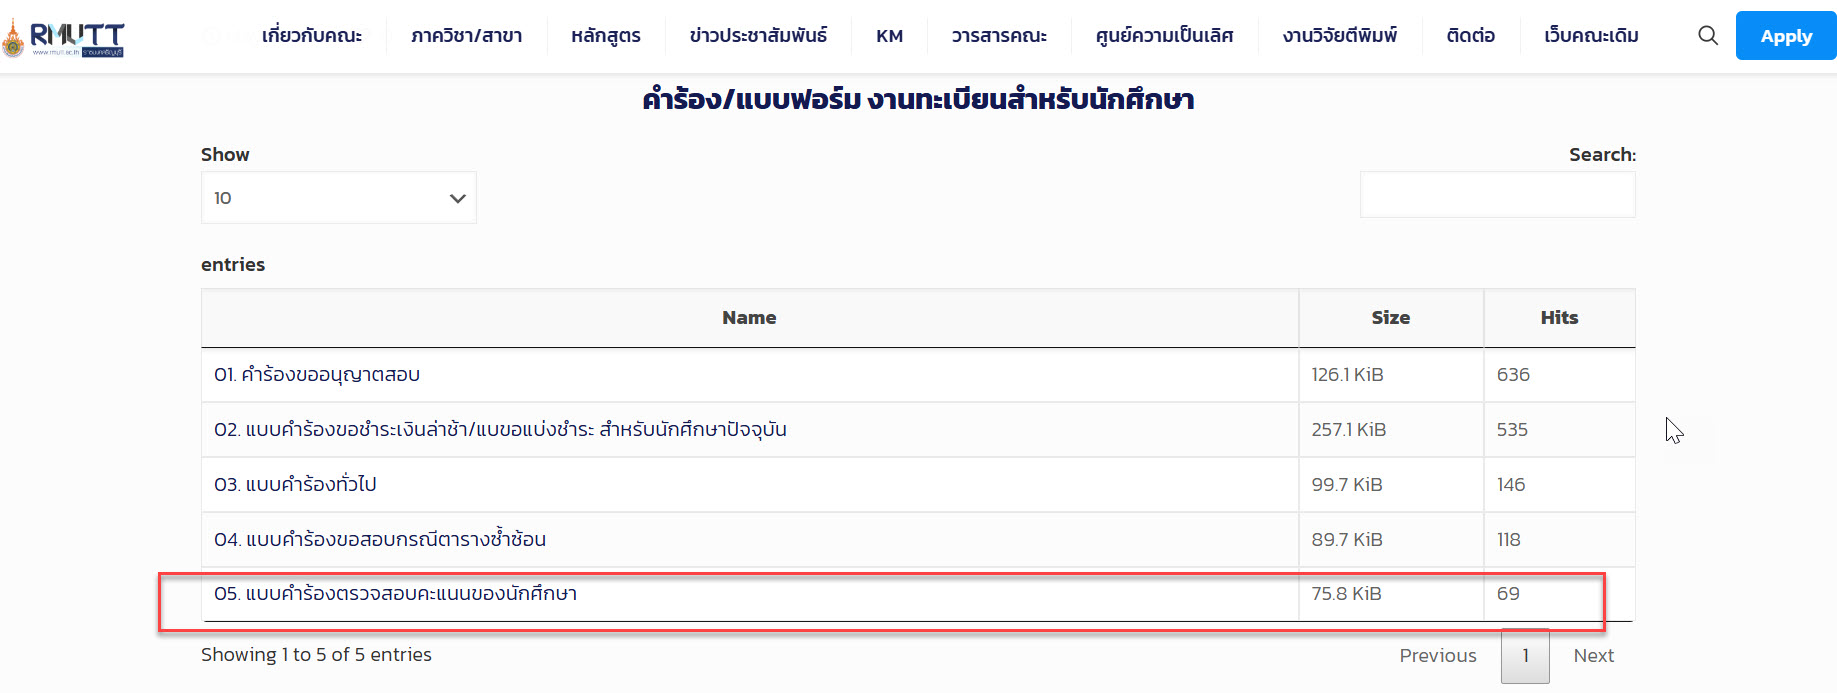
\includegraphics[width=\textwidth]{Pic4.2-1.jpg}
		\caption{หน้าเว็บไซต์เพื่อดาวน์โหลดเอกสารข้อร้องเรียนหรืออุทธรณ์ผลการประเมิน}
\end{figure}
\\
\noindent
ขั้นตอนการอุทธรณ์ผลการประเมิน
\begin{enumerate}
\item ยื่นคำร้องที่เจ้าหน้าที่ธุรการสาขา ในวันและเวลาราชการ โดยวันสุดท้ายที่จะสามารถยื่นเรื่องได้จะต้อง
ไม่เกิน 7 วันทำการนับจากวันสุดท้ายที่คณะส่งค่าระดับคะแนนตามกำหนดการของสำนักส่งเสริมวิชาการและ
งานทะเบียน (สวท.)
\item ขอดูได้เป็นรายบุคคลเท่านั้น โดยธุรการสาขานัดหมายนักศึกษาให้มาดูเอกสารประกอบการตรวจสอบ
หลังจากยื่นคำร้องในวันทำการถัดไปในกรณีที่ยื่นคำร้องก่อนเวลา 12.00 น. หรือในอีก 2 วันทำการถัดไปในกรณี
ที่ยื่นคำร้องหลังเวลา 12.00 น.
\item ธุรการสาขาประสานงานกับคณะกรรมการการอุทธรณ์ที่ได้รับการแต่งตั้งจากสาขาวิชา ซึ่งคณะกรรมการชุดดังกล่าวไม่มีส่วนเกี่ยวข้องกับอาจารย์ผู้สอนรายวิชาที่นักศึกษาได้ยื่นเรื่องอุทธรณ์ เพื่อจัดเตรียมเอกสารและนัดหมายเวลาสำหรับการเข้า
ตรวจสอบคะแนนของนักศึกษา ทั้งนี้ให้ธุรการสาขาดำเนินการหลังจากได้รับคำร้องจากนักศึกษาทันที
\item ผู้สอนจัดเตรียมกระดาษคำตอบของนักศึกษา เฉลย และเกณฑ์การให้คะแนนของข้อสอบในรายวิชา
นั้น ๆ ให้แก่คณะกรรมการการอุทธรณ์ที่ได้รับการแต่งตั้งจากสาขาวิชา
\item นักศึกษาเข้าพบธุรการสาขา และคณะกรรมการการอุทธรณ์ที่ได้รับการแต่งตั้งจากสาขาวิชาเพื่อตรวจสอบเอกสาร โดยไม่อนุญาตให้จด บันทึกภาพถ่ายหรือวีดีโอขณะทำการตรวจสอบเอกสาร
\item หากนักศึกษาไม่ยอมรับผลคะแนนสอบหลังจากทำการตรวจสอบคะแนนแล้ว ให้ธุรการสาขาส่งเรื่องต่อ
ให้กับงานทะเบียนและวัดผล ฝ่ายวิชาการ เพื่อดำเนินการแต่งตั้งคณะกรรมการเพื่อตรวจสอบการให้คะแนนของ
ผู้สอนอีกครั้ง โดยมีคณะกรรมการในการดำเนินการ 3 ท่าน คือ 1) รองคณบดีฝ่ายวิชาการ 2) หัวหน้างาน
ทะเบียนและวัดผล และ 3) หัวหน้าภาควิชา/สาขาวิชา หรือตัวแทนคณะกรรมการหลักสูตรที่เกี่ยวข้อง
\item งานทะเบียนและวัดผล ฝ่ายวิชาการ ดำเนินการนัดหมายคณะกรรมการในการตรวจสอบ อาจารย์ผู้สอนนักศึกษา และธุรการสาขา เพื่อดำเนินการตรวจสอบต่อไป และดำเนินการให้เสร็จสิ้นภายใน 3 วันทำการ
\end{enumerate}

ในปีการศึกษา 2566 ไม่มีนักศึกษาดำเนินการอุทธรณ์ผลการประเมิน 

\begin{doclist}
	\docitem{แบบคำร้องขอตรวจสอบคะแนนของนักศึกษา}
\end{doclist}


%%%%%%% 4.3 %%%%%%%%%%%%%%%%%%%%%%%
\subcriteria{The assessment standards and procedures for student progression and degree completion, are shown to be explicit, communicated to students, and applied consistently.}

หลักสูตรมีเกณฑ์การจบการศึกษาดังข้อบังคับ ระเบียบ และประกาศ ที่เกี่ยวข้องกับการจัดการศึกษาของมหาวิทยาลัยเทคโนโลยีราชมงคลธัญบุรี ต่อไปนี้
\begin{itemize}
 \item ข้อบังคับมหาวิทยาลัยเทคโนโลยีราชมงคลธัญบุรีว่าด้วยการศึกษาระดับปริญญาตรี พ.ศ. 2550
\item	ข้อบังคับมหาวิทยาลัยเทคโนโลยีราชมงคลธัญบุรีว่าด้วยการศึกษาระดับปริญญาตรี (ฉบับที่ 2) พ.ศ. 2556
\item	ข้อบังคับมหาวิทยาลัยเทคโนโลยีราชมงคลธัญบุรีว่าด้วยการจัดการระบบสหกิจศึกษา พ.ศ. 2550
\item	ระเบียบมหาวิทยาลัยเทคโนโลยีราชมงคลธัญบุรีว่าด้วยการเทียบโอนผลการเรียน พ.ศ. 2562
\item	ประกาศมหาวิทยาลัยเทคโนโลยีราชมงคลธัญบุรี เรื่อง เกณฑ์การวัดและประเมินผลการศึกษาระดับปริญญาตรี
\item	ประกาศมหาวิทยาลัยเทคโนโลยีราชมงคลธัญบุรี เรื่อง เกณฑ์มาตรฐานความสามารถทางภาษาอังกฤษของนักศึกษาระดับปริญญาตรีก่อนสำเร็จการศึกษา พ.ศ. 2560
\item	ประกาศมหาวิทยาลัยเทคโนโลยีราชมงคลธัญบุรี เรื่อง เกณฑ์มาตรฐานความสามารถทางภาษาอังกฤษของนักศึกษาระดับปริญญาตรีก่อนสำเร็จการศึกษา (ฉบับที่ 2) พ.ศ. 2562
\end{itemize}
ซึ่งหลักสูตรมีการสื่อสารไปยังนักศึกษา ดังนี้
\begin{enumerate}
\item แจ้งในวันปฐมนิเทศนักศึกษาใหม่
\item แจ้งในคู่มือนักศึกษา
\item อาจารย์ที่ปรึกษาของแต่ละชั้นปีแจ้งในวันโฮมรูม
\item แจ้งใน มคอ.2
\end{enumerate}

ทั้งนี้หลักสูตรกำหนดให้อาจารย์ที่ปรึกษาติดตามความก้าวหน้าและการสำเร็จการศึกษาของนักศึกษาให้เป็นไปตามข้อบังคับ ระเบียบ และประกาศ ที่เกี่ยวข้องกับการจัดการศึกษาของมหาวิทยาลัยเทคโนโลยีราชมงคลธัญบุรี 
 
\begin{doclist}
	\docitem{ข้อบังคับ ระเบียบ และประกาศ ที่เกี่ยวข้องกับการจัดการศึกษาของมหาวิทยาลัยเทคโนโลยีราชมงคลธัญบุรี}
	\docitem{คู่มือนักศึกษา}
	\docitem{มคอ.2}
\end{doclist}

%%%%%%% 4.4 %%%%%%%%%%%%%%%%%%%%%%%
\subcriteria{The assessments methods are shown to include rubrics, marking schemes, timelines, and regulations, and these are shown to ensure validity, reliability, and fairness in assessment.}

เพื่อให้เกิดความมั่นใจว่าการวัดและประเมินผลนักศึกษามีความถูกต้อง เชื่อถือได้ และเป็นธรรม โดยหลักสูตรมีการดำเนินการดังนี้ 
\begin{enumerate}
\item ทุกรายวิชามีการแจ้งกำหนดการ ข้อกำหนดต่าง ๆ ที่นักศึกษาต้องปฏิบัติตาม และเกณฑ์ในการวัดและประเมินผลของรายวิชาให้นักศึกษาทราบอย่างละเอียดและครบถ้วนตั้งแต่คาบแรกของการเรียนการสอน
\item ทุกรายวิชามีการใช้แบบประเมินผลทั้งแบบ rubrics หรือ marking schemes ที่สอดคล้องตามบริบทของรายวิชาที่มีการเรียนการสอน ดังนี้

\begin{itemize}
	\item[2.1] รายวิชาชีพที่มีการทดสอบโดยข้อสอบอัตนัย อาจารย์ผู้สอนจะมีการทำเฉลยและเกณฑ์การให้คะแนน หรือ marking schemes เพื่อใช้ในการตรวจข้อสอบ เช่น รายวิชา Abstract Algebra ดังรูปภาพที่ \ref{Picture:Marking Schemes}
	\begin{figure}[h!]
		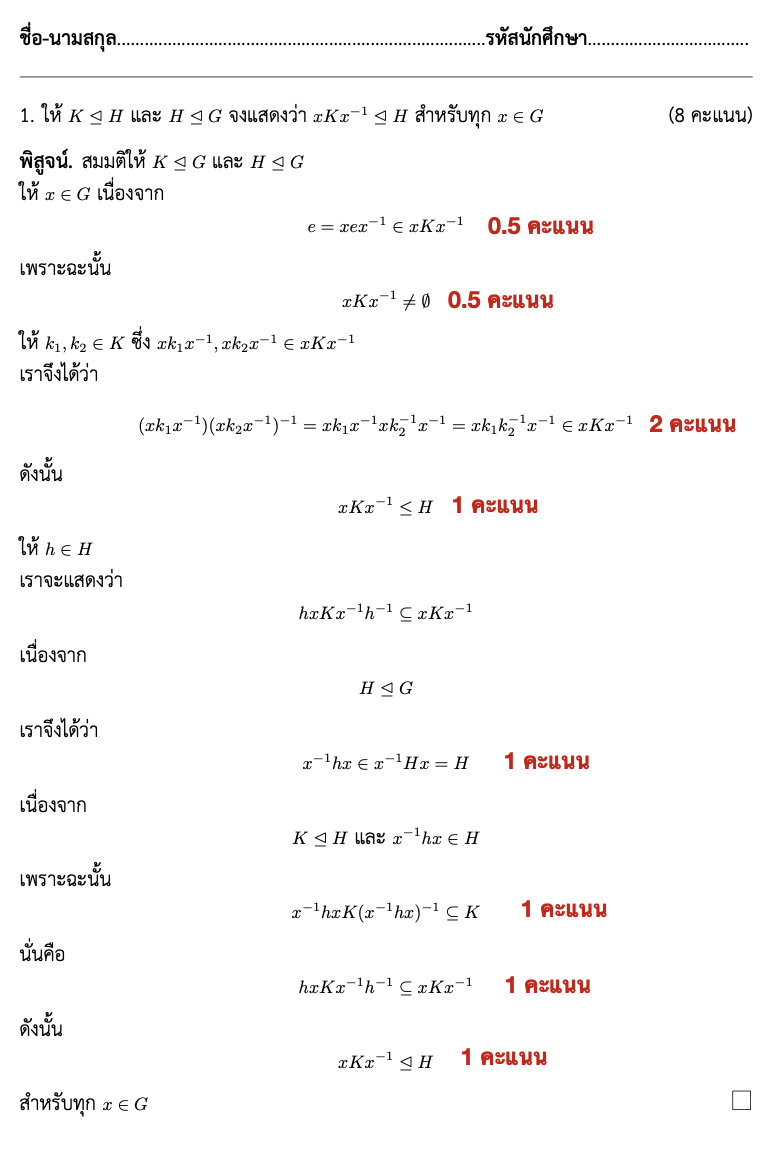
\includegraphics[width=\textwidth]{Abstract Algebra Points}\\
		\caption{ตัวอย่าง Marking Schemes ของข้อสอบรายวิชา Abstract Algebra  }
		\label{Picture:Marking Schemes}
	\end{figure}
\newpage
	\item[2.2] 
	หลักสูตรใช้ Scoring Rubrics สำหรับรายวิชาชีพที่มีการประเมินผลการนำเสนอผลงาน โดยหลักสูตรได้จัดทำ Scoring Rubrics สำหรับให้คะแนนการนำเสนอผลงาน ซึ่งผ่านการพิจารณาเห็นชอบจากที่ประชุมอาจารย์ผู้รับผิดชอบหลักสูตรและอาจารย์ผู้สอน เพื่อใช้เป็นเกณฑ์กลางในการประเมินผล พร้อมทั้งแจ้งให้นักศึกษาทราบ
\end{itemize}
\end{enumerate}


\begin{doclist}
	\docitem{marking schemes ของแบบทดสอบย่อยรายวิชา Abstract Algebra}
	\docitem{Scoring Rubrics สำหรับการประเมินผลการนำเสนอผลงาน}
\end{doclist}

%%%%%%% 4.5 %%%%%%%%%%%%%%%%%%%%%%%
\subcriteria{The assessment methods are shown to measure the achievement of the expected learning outcomes of the programme and its courses.}
\noindent
{\bf วิธีการประเมินการบรรลุ PLOs}

\printprogram{} ได้กำหนดวิธีการประเมินผลการบรรลุผลลัพธ์การเรียนรู้ที่คาดหวังของหลักสูตร  (PLOs) โดยใช้แบบสอบถาม ``แบบประเมินการบรรลุผลลัพธ์การเรียนรู้ที่คาดหวังของหลักสูตร (PLOs)"  ให้นักศึกษาชั้นปีสุดท้ายประเมินตนเอง

ในปีการศึกษา 2566 \printprogram{} ยังไม่มีนักศึกษาชั้นปีสุดท้ายจึงยังไม่มีการดำเนินการในประเด็นนี้\\

\noindent
{\bf วิธีการประเมินการบรรลุ CLOs}

\printprogram{} ได้กำหนดวิธีการประเมินผลการบรรลุผลลัพธ์การเรียนรู้ที่คาดหวังของรายวิชา  (CLOs) โดยใช้แบบสอบถาม ``แบบประเมินการบรรลุผลลัพธ์การเรียนรู้ที่คาดหวังของรายวิชา (CLOs)"  ให้นักศึกษาที่เรียนในรายวิชาประเมินตนเอง
แล้วนำผลการประเมินตนเองของนักศึกษามาวิเคราะห์และพิจารณาเพื่อใช้ในการปรับปรุงวิธีการสอนและการประเมินผลในภาคการศึกษา/ปีการศึกษาต่อไป
\begin{doclist}
	\docitem{แบบประเมินการบรรลุผลลัพธ์การเรียนรู้ที่คาดหวังของหลักสูตร (PLOs)}
	\docitem{แบบประเมินการบรรลุผลลัพธ์การเรียนรู้ที่คาดหวังของรายวิชา (CLOs)}
	\docitem{รายงานผลการประเมินการบรรลุผลลัพธ์การเรียนรู้ที่คาดหวังของรายวิชา (CLOs) ประจำปีการศึกษา 2566}
\end{doclist}

%%%%%%% 4.6 %%%%%%%%%%%%%%%%%%%%%%%
\subcriteria{Feedback of student assessment is shown to be provided in a timely manner.}

หลักสูตรกำหนดให้อาจารย์ผู้สอนทุกรายวิชามีการให้ข้อมูลย้อนกลับ (Feedback) กับนักศึกษาทุกครั้งที่มีการประเมินผล เพื่อให้นักศึกษาทราบ  และนำไปปรับปรุงการเรียนรู้ในรายวิชา โดยการให้ข้อมูลย้อนกลับมีการดำเนินการดังนี้
\begin{enumerate}
	\item อาจารย์ผู้สอนทุกรายวิชาแจ้ง คะแนนสอบกลางภาค คะแนนทดสอบย่อย/คะแนนชิ้นงาน/คะแนนการนำเสนอ รวมถึงมีการเฉลยแบบทดสอบ/ การให้ข้อเสนอแนะข้อควรปรับปรุงในการนำเสนอหรือการสร้างชิ้นงาน โดยมีการแจ้งคะแนนทั้งหมดในระหว่างภาคการศึกษาเพื่อให้นักศึกษาสามารถประเมินผล และวางแผนการศึกษาของตนเองได้ก่อนกำหนดการถอนรายวิชา (W)
	\item วิชาโครงงาน มีการแจ้งข้อมูลย้อนกลับโดยอาจารย์ที่ปรึกษาโครงงานในระหว่างจัดทำโครงงาน และ มีการแจ้งข้อมูลย้อนกลับโดยกรรมการในการประเมินเล่มโครงงานและการนำเสนอโครงงานเพื่อให้นักศึกษาสามารถนำข้อมูลนั้น ๆ ไปปรับปรุงและพัฒนาผลงาน
	\item วิชาสัมมนาทางคณิตศาสตร์ หลักสูตรมีการแต่งตั้งกรรมการประเมินการนำเสนอการถอดบทเรียนของนักศึกษาและอาจารย์ที่ปรึกษาสำหรับแนะนำการถอดบทเรียนกับนักศึกษา โดยในการนำเสนอแต่ละครั้งกรรมการจะสอบถามและให้คำแนะนำระหว่างการนำเสนอ
เพื่อให้นักศึกษาสามารถนำข้อมูลนั้น ๆ ไปพัฒนาและปรับปรุงในการสัมมนาในครั้งถัดไป
\end{enumerate}


%%%%%%% 4.6 %%%%%%%%%%%%%%%%%%%%%%%
\subcriteria{The student assessment and its processes are shown to be continuously reviewed and improved to ensure their relevance to the needs of industry and alignment to the expected learning outcomes.}

\printprogram{} มีระบบในการทบทวนเกณฑ์ที่ใช้ในการประเมินผลนักศึกษา เพื่อให้สอดคล้องกับความต้องการของภาคอุตสาหกรรม ผลลัพธ์การเรียนรู้ที่คาดหวังของรายวิชา (CLOs) และวัตุประสงค์ของรายวิชา โดย
\begin{enumerate}
	\item หลักสูตรมีการทวนสอบผลสัมฤทธิ์ของนักศึกษาตามผลลัพธ์การเรียนรู้ที่คาดหวังของรายวิชา (CLOs) ทุกรายวิชาชีพที่เปิดสอนในแต่ละภาคเรียน โดย
	\begin{itemize}
		\item แต่งตั้งคณะกรรมการทวนสอบฯ
		\item คณะกรรมการทวนสอบฯ ดำเนินการทวนสอบหลังสิ้นภาคเรียน 
		\item คณะกรรมการทวนสอบฯ รายงานผลการทวนสอบให้หลักสูตรทราบ และแจ้งผลการทวนสอบพร้อมทั้งข้อเสนอแนะให้กับอาจารย์ผู้รับผิดชอบรายวิชา และอาจารย์ผู้สอนทราบเพื่อนำไปปรับปรุงต่อไป 
	\end{itemize}
	\item หลักสูตรมีการส่ง มคอ.3 ของรายวิชาที่เกี่ยวข้องกับภาคอุตสาหกรรม ให้สถานประกอบการในภาคอุตสาหกรรมพิจารณาความเหมาะสมของวิธีการประเมินผลก่อนเปิดภาคเรียน เพื่อให้การประเมินผลในรายวิชามีความสอดคล้องตามความต้องการของภาคอุตสาหกรรม
\end{enumerate}
{\bf ผลการดำเนินงาน}

 หลักสูตรมีการทวนสอบทุกรายวิชาชีพที่เปิดสอนในปีการศึกษา 2566 จำนวน 27 รายวิชา แบ่งเป็น
\begin{enumerate}
	\item[] - ภาคเรียนที่ 1/2566 จำนวน 9 รายวิชา
	\item[] - ภาคเรียนที่ 2/2566 จำนวน 18 รายวิชา
\end{enumerate}
ผลการทวนสอบพบว่าทุกรายวิชามีการประเมินผลที่สอดคล้องกับผลลัพธ์การเรียนรู้ของรายวิชา(CLOs)

นอกจากนี้ เพื่อให้การประเมินผลมีความสอดคล้องตามความต้องการของภาคอุตสาหกรรม หลักสูตรได้ส่ง มคอ.3 รายวิชาระเบียบวิธีเชิงตัวเลขเบื้องต้นและรายวิชาระบบฐานข้อมูล ให้ผู้เชี่ยวชาญจากภาคอุตสาหกรรมให้ข้อเสนอแนะเกี่ยวกับการประเมินผลในรายวิชาดังกล่าว โดยมีข้อเสนอแนะคือ หลักสูตรควรเน้นให้มีการประเมินผลในภาคปฏิบัติให้มากขึ้นเพื่อเป็นการการันตีได้ว่าหลังจากเรียนแล้วนักศึกษาสามารถนำไปใช้ได้จริง
ผู้สอนในรายวิชาาระเบียบวิธีเชิงตัวเลขเบื้องต้นและรายวิชาระบบฐานข้อมูลได้นำข้อเสนอแนะมาปรับปรุงการประเมินผลโดยมีการเพิ่มการประเมินผลในภาคปฏิบัติทั้งสองรายวิชา

\begin{doclist}
	\docitem{รายงานผลการทวนสอบปีการศึกษา 2566}
	\docitem{ข้อเสนอแนะการประเมินผลจากภาคอุตสาหกรรม}
\end{doclist}


